\section{Tools}
    Python is an interpreted, high-level programming language. Python is an object-oriented programming language and really dynamic and flexible. It is believe that python is a minimalistic language. Developer can really focus on the real issue, not its syntax~\cite{GGGG}. Further more, Python is used too solve the problem in this article is because the variety in library. Python support very good in process large amount of data.
    
    Beside amazing feature that come original from Python, Python also support the tools and famous library that widely use in machine learning and more specific in this case is recursive neural network. In this thesis, I will use scipy for denoising the signal and keras to make a recursive neural network.

    \subsection{MNE-python}
    MNE is a very powerful tool to exploring, visualizing, and analyzing human neurophysiological data: MEG, EEG, sEEG, ECoG, and more. Most of the tool in this Python application we will not use, but to simplify the process of visualize signal before and after we apply filter, this tool is very convenient. MNE-tool tends to be a great library in this major, but in this article, we will not use the available preprocessing tools that available in the tools, but only use it to visualize the input and also the preprocessed signal before we do any further process~\cite{MNE}.
    
    \subsection{Keras}
    Most of the deep learning library in the market right now receive supports by some large companies. For example Facebook has Pytorch and Caffe2 or Microsoft has CNTK. However, we will use the most famous library from Google, whichs is Keras base on Tensorflow.
    
    The figure below illustrates the market share of Tensorflow and Keras from Google\cite{marketshare}. As you can see in the figure 2.1, Tensorflow and Keras have very large amount of user than any other libraries because of the simplicity that the tool bring to us. Thus, We will use Keras as the high-level library with the low-level is Tensorflow to make it simple. Keras has much simple syntax than Tensorflow itself.
    
    \begin{figure}[h]
        \centering
        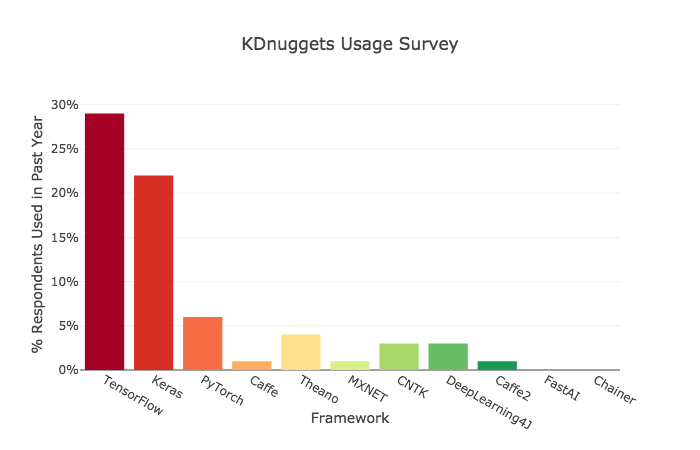
\includegraphics[width = 0.9\textwidth]{images/KERA_usage.png} 
        \caption{KDnuggets usage survey}
        \label{fig:marketshare}
    \end{figure}
    
    \subsection{Some famous python library}
    Pandas, Numpy and Matplotlib are very famous libraries in Python. We could say that these libraries are buildings the fundamentals of the successful that the reason we use Python for. Beside of the fundamental library, for this specific article, The list below show some more of the library that we will use in this problem.
    
    \begin{itemize}
        \item Scipy
        
        In this article, we will use Scipy for caculate the Z-score of the datasets, and use Z-score as a outliers detection in order to remove these artifact that appeared in the signal.
        \item Random
        
        The random library is used to mix the labeled data that we feed to the neural network. If we do not mix the divided dataset with each others, it is believe that the model is not so good in learning things from the signal we have.
        \item Pickle
        
        After we have the preprocessed data complete, We do not want to run that every time we use the processed signal again, so Pickle will export the data we processed to a file for later usage.
        \item Scikit learn
        
        The Scikit learn library does a important roll to normalize the signal which is raise the learning rate.
    \end{itemize}
    
\section{Datasets}
    The data I use in this article was provide by professor Sebastian Basterrech. The dataset contains 19 different electrodes, which is FP1-AVE,FP2-AVE, F3-AVE, F4-AVE, C3-AVE,  C4-AVE, P3-AVE, P4-AVE, O1-AVE,  O2-AVE, F7-AVE, F8-AVE, T3-AVE, T4-AVE, T5-AVE, T6-AVE, Fz-AVE, Cz-AVE and Pz-AVE. Each electrode have a specific position in the head, and the name represent its location. The number of electrode is the 10-20 international electrode system.
    
    This version has been reduced compare to the full electrode version. If we put too much electrode to record the electrical signal, It will be have intersections between electrodes and the output results might not so correct to determine which electrode is belong to which region of the brain.
    
    There are also almost 17000 data point, so to display all the data I use is impossible. The figure below only represent 15 first line of the data we use in this article. I can show this short version by using head\(\) function built-in in pandas. The first data point will be in zero for more equal between electrodes.

    \begin{figure}[h]
        \centering
        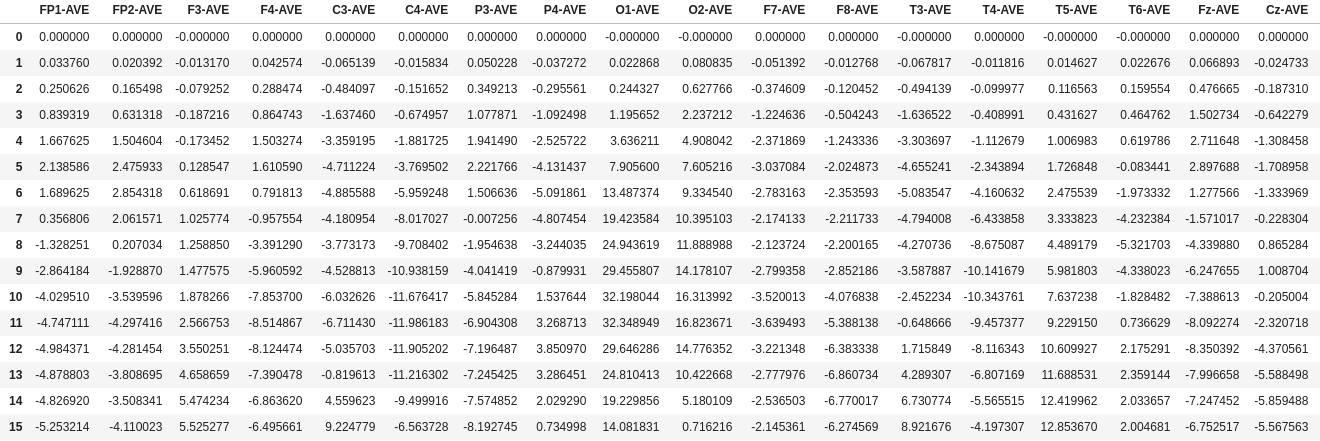
\includegraphics[width=1\textwidth]{images/data.png}
        \caption{First 15 data points}
    \end{figure}

    You can see more details the place that these electrodes sit on the skull in order to know the location of the name of the electrodes in chapter 1. The electrode is divided into 4 classes as we discussed before. The first character of the name contain the location that the electrode measure.
    
    \begin{itemize}
        \item Class 0: Frontal lobe (F) 
        
        including FP1-AVE, FP2-AVE, F3-AVE, F4-AVE, F7-AVE, F8-AVE, Fz-AVE
        \item Class 1: Cerebellum (C) 
        
        including C3-AVE, C4-AVE, Cz-AVE
        \item Class 2: Temporal lobe (T) 
        
        including T3-AVE, T4-AVE, T5-AVE, T6-AVE
        \item Class 3: Parietal lobe (P) and Occipital lobe (O) 
        
        including P3-AVE, P4-AVE, Pz-AVE, O1-AVE,  O2-AVE
    \end{itemize}
    
    